
Any residual image background will bias derived galaxy magnitudes. We
use a custom background subtraction algorithm to take out any residual
large-scale varying background. We start with stacked images produced
by {\sc MutiDrizzle}. The individual images are already background
subtracted prior to the {\sc MultiDrizzle} process, but we find that
the stacked images have a small positive mean background.

Objects are detected with Source Extractor 
\citep[{\sc SExtractor};][]{bertin96a} using the standard
one-pass, single-image mode. {\sc SExtractor} is allowed to determine
its own spatially-varying image background, solely for the purposes of
object detection and object geometry. The relevant detection
parameters are given in Table~\ref{tab:sextractor}. A mask is then
created based on the {\sc SExtractor} catalog -- all pixels inside an
object's MAG\_AUTO aperture are masked. In particular, note that
PHOT\_AUTOPARAMS is set to [8.0, 3.3]. This means that each object is
masked out to 8 times its Kron radius. (See \S\ref{sec:lum_correction}
below for a more detailed discussion of MAG\_AUTO and Kron radius.)
The radius used for masking objects is a trade-off between ensuring
that all galaxy light is masked and having any pixels left for
background determination. With these settings, typically between
half and two thirds of the pixels in the image are masked
(Fig.~\ref{fig:background}). The background is then determined in
$50 \times 50$ pixel boxes (all pixels in each box are assigned the
same background). At the location of each box, we take all unmasked
pixels in a $500 \times 500$ pixel box. If there are not ``enough''
unmasked pixels in this box to determine a reliable background, we
expand the box until there are enough. When there are enough, we take
the mean of the unmasked pixels as the background for all pixels in
the $50 \times 50$ pixel box.

\begin{table}
\caption{{\sc SExtractor} parameters for galaxy detection and photometry\label{tab:sextractor}}
\begin{center}
\begin{footnotesizetabular}{lcccc}

\hline
\hline
               & Object Masking       & & \multicolumn{2}{c}{Object Detection} \\
\cline{4-5}
Parameter Name & for Image Background & & Cold Value    & Hot Value           \\
\hline
FILTER           & Y        & & Y       & Y\\
CLEAN            & Y        & & Y       & Y\\
CLEAN\_PARAM     & 1.2      & & 1.2     & 1.2\\
BACK\_TYPE       & AUTO     & & AUTO    & AUTO\\
BACK\_SIZE       & 120      & & 5       & 4\\
BACK\_FILTERSIZE & 4        & & 5       & 4\\
DETECT\_MINAREA  & 5        & & 50      & 5\\
DETECT\_THRESH   & 1.65     & & 3.0     & 1.65\\
ANALYSIS\_THRESH & 1.65     & & 3.0     & 1.65\\
DEBLEND\_NTHRESH & 64       & & 64      & 64\\
DEBLEND\_MINCONT & 0.05     & & 0.007   & 0.05\\
PHOT\_AUTOPARAMS & 8.0, 3.3 & & 5.0,0.0 & 5.0,0.0\\
\hline

\end{footnotesizetabular}
\end{center}
\end{table} 


\begin{figure}[tp]
\begin{center}
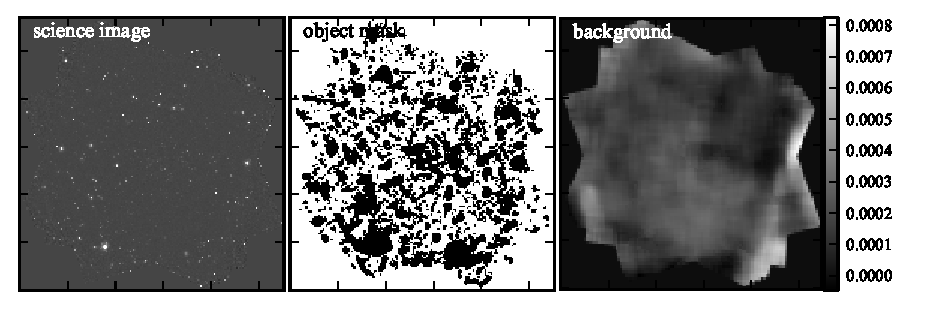
\includegraphics{figures/clrate/images_A.eps}
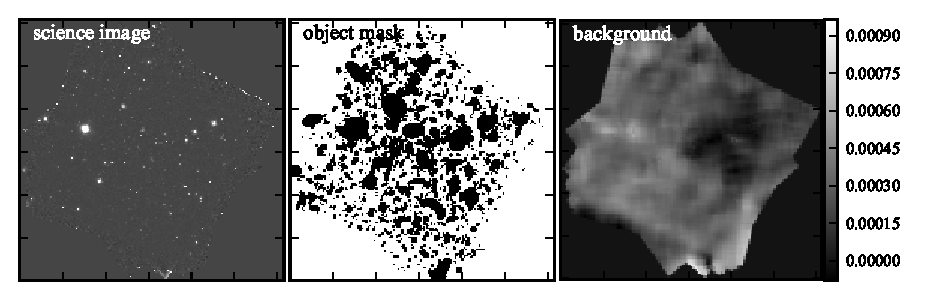
\includegraphics{figures/clrate/images_B.eps}
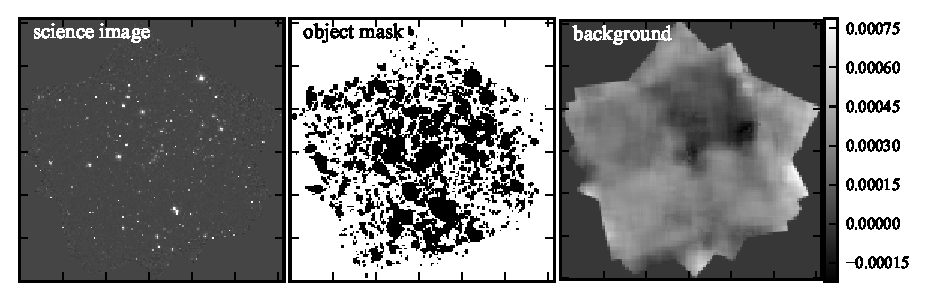
\includegraphics{figures/clrate/images_C.eps}
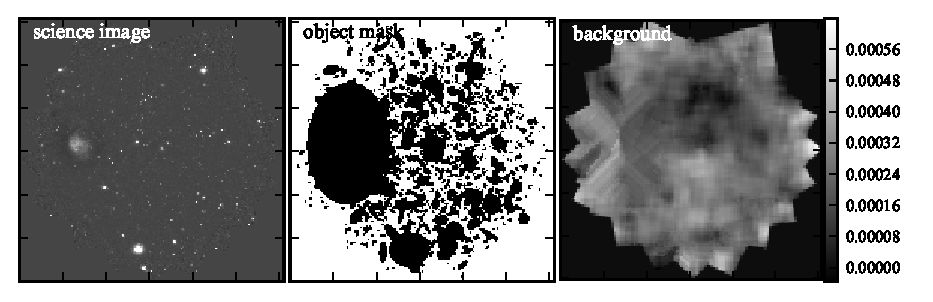
\includegraphics{figures/clrate/images_E.eps}
\end{center}
\caption[Image background determination examples]{Examples of background
  determination for the $z_{850}$ image of clusters A, B, C and E
  (descending by row). The columns are the science image (left),
  object mask (center), and derived image background (right). The
  scale is counts~s$^{-1}$~pixel$^{-1}$ in the background
  image.\label{fig:background}}
\end{figure}

In Fig.~\ref{fig:background} (right column) one can see that the
images typically have a positive flux background.  For reference,
summed over a 10 (20) pixel radius aperture a flux of 0.0005
counts~s$^{-1}$~pixel$^{-1}$ is equivalent to a flux of 0.157 (0.628)
counts~s$^{-1}$, or a $z_{850} = 26.87$ (25.37).  The other feature
that stands out is a quadrant effect. For clusters A, B and C, one
quadrant of the image has a background that is clearly lower than the
other quadrants. The effect is less obvious in clusters where the
component images had a wider range of orientations (like cluster E).

%Cluster E is an interesting case, due to the presence of a very
%extended object left of image center. {\sc SExtractor} correctly
%identifies this as a single object, resulting in a large elliptical
%region being masked. In the background image, this results in
%characteristic diagonal streaks, due to the fact that the same pixels
%are being used to compute the background at different locations in
%the masked region. This is not generally a problem though: the
%background may not be as accurate at these locations, but it should
%still be unbiased.
